\documentclass[10pt, letterpaper]{article}
%\documentclass[english]{article}
\usepackage[a4paper, total={19cm, 25cm}]{geometry}
\usepackage{graphicx}
\usepackage{amsmath}
\usepackage{amssymb}
\usepackage{booktabs}
\usepackage{nicefrac}
\usepackage{multicol}
\usepackage{enumitem}
\usepackage{lipsum}% http://ctan.org/pkg/lipsum
\usepackage{algorithm}
\usepackage[algo2e]{algorithm2e} 
\usepackage{multirow}
\usepackage[pagebackref,breaklinks,colorlinks]{hyperref}
% \setlength{\parindent}{0pt}
% Support for easy cross-referencing
\usepackage[capitalize]{cleveref}
\crefname{section}{Sec.}{Secs.}
\Crefname{section}{Section}{Sections}
\Crefname{table}{Table}{Tables}
\crefname{table}{Tab.}{Tabs.}
\renewcommand\thesection{\Roman{section}}
\nocite{*}

\begin{document}
\begin{multicols*}{2}
\noindent %no alinea
Where $^M\mathbf{\boldsymbol{\hat{\rho}}}_{i}$ is the estimated four-wall room center obtained
from Section. IV-C and $\textit{f }(^M\boldsymbol{\tilde{\pi}}_{x_{a_{i}}}, ^M\boldsymbol{\tilde{\pi}}_{x_{b_{i}}}, ^M\boldsymbol{\tilde{\pi}}_{y_{a_{i}}}, ^M\boldsymbol{\tilde{\pi}}_{y_{b_{i}}})$ is the function mapping the four wall planes estimated to a fourwall room center using Eq. 4. The goal of this cost function is to maintain the structural consistency between the four planes forming the room.

$\textbf{\textit{Two-Wall Rooms}}$: We propose a similar cost function to
minimize room nodes and their two corresponding wall planes
as follows:
\begin{equation}
    \begin{aligned}
        {c}_{\textbf{\textit{k}}}(^M{\textbf{\textit{k}}}_{i}, \left[^M{\boldsymbol{\pi}}_{x_{a_{1}}},^M{\boldsymbol{\pi}}_{x_{b_{1}}},^M{\bf{c}}_{i}\right])\\
        =\sum_{t=1,i=1}^{T,K} ||^M{\hat{\textbf{\textit{k}}}_{i}} - \textit{f }( ^M{\boldsymbol{\tilde{\pi}}}_{x_{a_{1}}},^M{\boldsymbol{\tilde{\pi}}}_{x_{b_{1}}},^M{\bf{c}}_{i})||_{\boldsymbol{\bigwedge}_{\tilde{\textbf{\textit{k}}}_{i,t}}}^2
    \end{aligned}
    \label{eq:zn}
\end{equation}
$^M\textbf{c}_i$ is the cluster center, which is kept constant during the optimization, and $^M\hat{k}_i$ is the estimated two-wall
room center in $\textit{x}$ direction obtained from Section. IV-C. $\textit{f }( ^M{\boldsymbol{\tilde{\pi}}}_{x_{a_{1}}},^M{\boldsymbol{\tilde{\pi}}}_{x_{b_{1}}},^M{\bf{c}}_{i})$ maps the two wall planes and its
cluster center to a room center using Eq. 5. The cost function to
minimize two-wall rooms in $\textit{y}$ direction follows \cref{eq:zn}  for wall
planes $(^M\boldsymbol{{\pi}}_{y_{a_{j}}}, ^M\boldsymbol{{\pi}}_{y_{b_{j}}})$ and cluster center $^M\mathbf{c}_j$. Duplicate
wall plane nodes identified during the four-wall or two-wall
room segmentation are constrained by a factor minimizing the
difference between their respective parameters.

\textbf{Floors.} The floor node consists of the center of the current floor level calculated from the floor segmentation (Section. IV-D). We add a cost function between the floor node and
all the mapped four-wall rooms at that floor level as follows:
\begin{equation}
    \begin{aligned}
        {c}_{\xi}(^M \boldsymbol{\xi}_i,^M \boldsymbol{\rho}_i)= \sum_{t=1,i=1,j=1}^{T,F,S} ||^M{\boldsymbol{\hat{\xi}}_{\xi_i,\rho_j}} - \textit{f }(^M \boldsymbol{\xi}_i,^M \boldsymbol{\rho}_j)||_{\boldsymbol{\bigwedge}_{\boldsymbol{\tilde{\xi}}_{i,t}}}^2
    \end{aligned}
    \label{eq:cd}
\end{equation}
where $^M\boldsymbol{\xi}_{\xi_i,\rho_j}$ j stands for the relative distance between the
floor $\textit{i}$ with center $\boldsymbol{\xi}_i$ and the four-wall room $\textit{j}$ with center $\mathbf{\boldsymbol{\rho}}_{j}$, and $\textit{f }(^M \boldsymbol{\xi}_i,^M \boldsymbol{\rho}_i)$ maps the relative distance between the
centers of floor node and four-wall room node. Two-wall room
nodes are constrained with the floor node using the same \cref{eq:cd} While the robot navigates in the surroundings and discovers
new wall planes, the estimate of the floor node might change
due to the insertion of such planes into the map. If the current
floor center calculated from the new wall planes gets updated
beyond a threshold $\textit{t}_f$, the estimate of the floor node is updated
in the graph accordingly along with the relative distances
between the floors and all the rooms.
\section{EXPERIMENTAL RESULTS}
\begin{enumerate}[label=\Alph*.]
    \item Methodology
   
\end{enumerate}
 
 We validate $\textit{S-Graphs+}$ on simulated and real-world scenarios, comparing it against several state-of-the-art $\textbf{LiDAR SLAM}$ frameworks and the baseline $\textit{S-Graphs+}$. The experiments cover
a wide array of scenes, from construction sites to office spaces,
and use data recorded in-house and from the public TIERS
dataset. We report standard error metrics for the map and
trajectory estimations (RMSE and ATE) as well as qualitative
results. For comparing the room detection of $\textit{S-Graphs+}$ TABLE I: Absolute Trajectory Error (ATE) [m], of $\textit{S-Graphs+}$
and relevant baselines on simulated data. Best results are
boldfaced, second best are underlined.
\begin{table}[H] %* pour centrer
    \centering
    \begin{tabular}{l|c|clccccc} %l pour alligner
    \hline
     $\textbf{Method}$ && $\textbf{Dataset}$\\
     \hline
     Mapping & Odometry & C1F0 & C1F2 & SE1 & SE2 & SE3 \\
     \hline
     HDL-SLAM [10] & VGICP [26] & 0.15 & $\underline{0.02}$ & 0.04 & 0.15 & 0.14 \\
     ALOAM [5] &ALOAM  & 0.10 & 0.09 & 0.16 & 0.32 & 0.20 \\
     MLOAM [9] &MLOAM  & 1.14 & 0.52 & 0.65 & 2.82 & 0.17 \\
     FLOAM [6] &FLOAM  & 0.11 & 0.15 & 0.15 & 0.24 & 0.76 \\
     LeGO-LOAM [7] & LeGO-LOAM & -&  -&  - & - & 0.73 \\
     S-Graphs [8]&  VGICP&  $\underline{0.07}$&  $\underline{0.02}$&  $\underline{0.03}$ & 0.17&  0.33 \\
     \hline
     S-Graphs+ (ours) & VGICP & 0.08 &  $\textbf{0.01}$&  $\textbf{0.02}$ & $\textbf{0.12}$ & $\textbf{0.05}$\\
     S-Graphs+ (ours) & FLOAM & $\textbf{0.05}$ &  0.03 & 0.15&  $\underline{0.14}$ & $\underline{0.12}$\\
     \hline

    \end{tabular}
    \caption{Mon premier tableau}
    \label{tab:my_1table}
\end{table}
against the heuristics in $\textit{S-Graphs}$, we report the precision and
recall of the four-walled and two-walled room detections in the
simulated environments, for which we have the ground truth
number of rooms defined in the architectural plans.

$\textbf{Simulated Data.}$ We conduct a total of five simulated
experiments. Two of them, $\textit{CF1}$ and $\textit{CF2}$, are generated from
the 3D meshes of two floors of actual architectural plans. The
other three, $\textit{SE1}$, $\textit{SE2}$, and $\textit{SE3}$, are performed in additional
simulated environments resembling typical indoor environments with different room configurations. Due to absence of
odometry from robot encoders, in all simulated experiments
the odometry is estimated only from LiDAR measurements.
For a fair validation, $\textit{S-Graphs+}$ is run using two different
odometry inputs, specifically VGICP [26] and FLOAM [6].

$\textbf{In-House Dataset.}$ In all our in-house data we utilize
the robot encoders for estimating the odometry. The first
two experiments, denoted as $\textit{C1F1}$ and $\textit{C1F2}$, are performed
on two floors of a construction site consisting of a single
house. Additionally, experiments are performed over larger
construction sites combining several houses. $\textit{C2F0}$, $\textit{C2F1}$,
and $\textit{C2F2}$ consist of three floors of an ongoing construction
site combining four individual houses. $\textit{C3F1}$, and C3F2 are
two combined houses, while $\textit{C4F0}$ is a basement area with
different storage rooms. $\textit{LC1}$ consists of an office environment
in which the robot traverses back and forth a long corridor.
To validate the accuracy of each method in all the real experi-
\begin{figure}[H]
    \centering
    \begin{tabular}{cccc}
    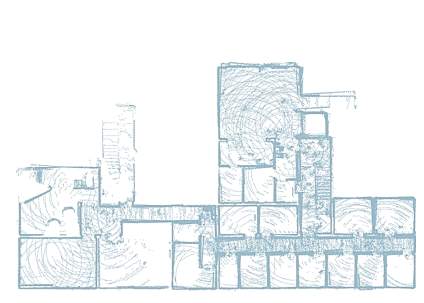
\includegraphics[width=3cm]{images/image_a.png} &
    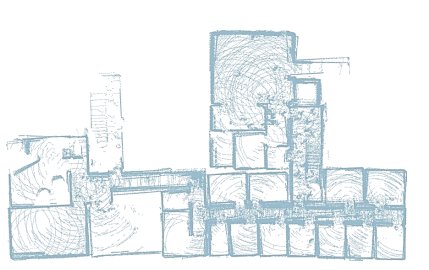
\includegraphics[width=3cm]{images/image_b.png} \\
    (a)S-Graphs+   & (b)  HDL-SLAM\\
    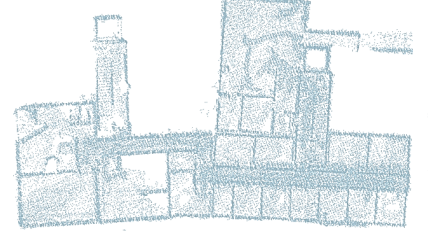
\includegraphics[width=3cm]{images/image_c.png} &
    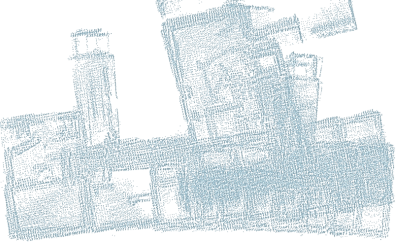
\includegraphics[width=3cm]{images/image_d.png}\\
    
     (c) ALOAM  & (d)  FLOAM\\ %~& pour espace car latex ne comprends pas les spaces, // fin
    
    
    \end{tabular}
    \caption{Maps by S-Graphs+ and baselines, in-house seq. $\it{C4F0.}$}
    \label{fig:my_label}
\end{figure}

{\small
\bibliographystyle{IEEEtran}
\bibliography{references}
}
\end{multicols*}
\end{document}

